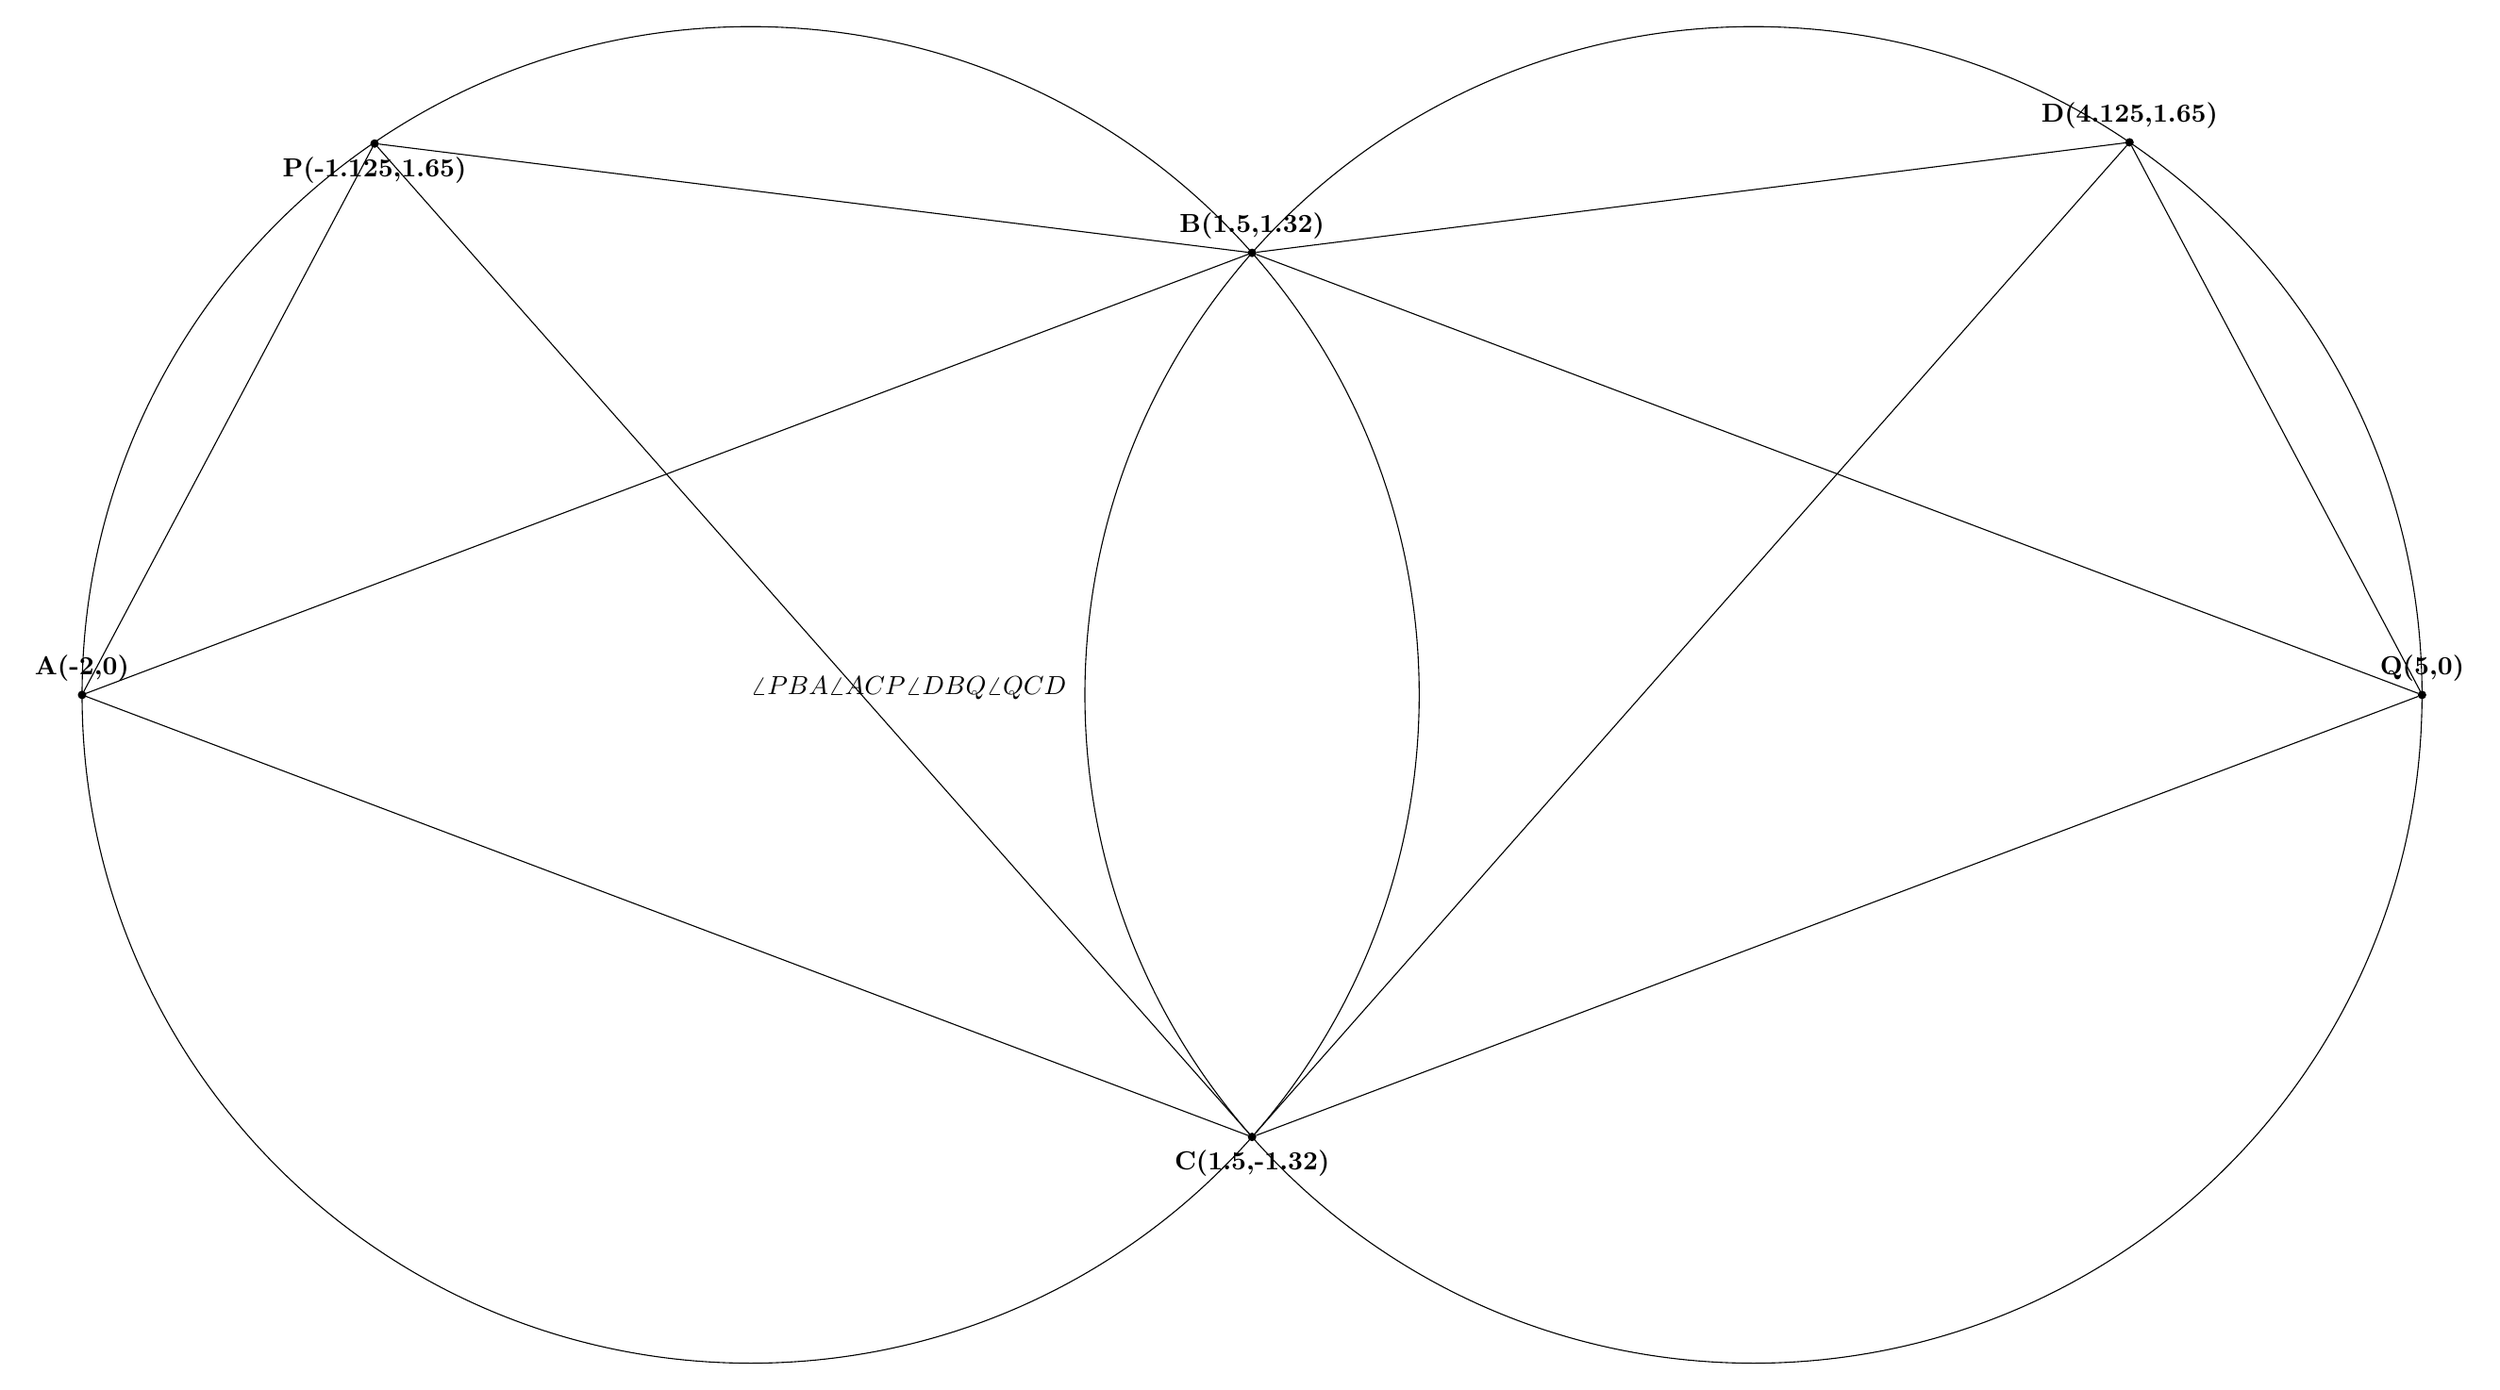
\begin{tikzpicture}[scale =4.5,>=stealth,point/.style = {draw, circle, fill = black, inner sep = 1pt},]
\draw (0,0)circle (2cm)(3,0) circle (2cm);
\node (A) at (-2,0)[point,label=above :$\textbf{A(-2,0)}$] {};
\node (P) at (-1.125,1.65)[point,label=below :$\textbf{P(-1.125,1.65)}$] {};
\node (B) at (1.5,1.3228756555322954)[point,label=above :$\textbf{B(1.5,1.32)}$] {};
\node (Q) at (5,0)[point,label=above :$\textbf{Q(5,0)}$] {};
\node (D) at (4.125,1.65359457)[point,label=above :$\textbf{D(4.125,1.65)}$] {};
\node (C) at (1.5,-1.3228756555322954)[point,label=below :$\textbf{C(1.5,-1.32)}$] {};
\draw (A)--(P)--(B)--(Q)--(C)--(P);
\draw (A)--(B)--(D)--(C)--(A);
\draw (D)--(Q);
\tkzMarkAngle[fill=black!45,size=.3,mark=](P,B,A)
\tkzLabelAngle[pos=-0.5](P,B,A){$\angle{PBA}$}
\tkzMarkAngle[fill=black!45,size=.3,mark=](P,C,A)
\tkzLabelAngle[pos=0.5](P,C,A){$\angle{ACP}$}

\tkzMarkAngle[fill=green!45,size=.3,mark=](Q,B,D)
\tkzLabelAngle[pos=0.5](Q,B,D){$\angle{DBQ}$}
\tkzMarkAngle[fill=green!45,size=.3,mark=](Q,C,D)
\tkzLabelAngle[pos=0.5](Q,C,D){$\angle{QCD}$}
\end{tikzpicture}

